% ---------
%  Compile with "./build.sh"
% --------

\documentclass[10pt]{article}
\usepackage{amsmath}
\usepackage[margin=1in]{geometry}
\usepackage{import}
\usepackage{amssymb}
\usepackage{float}
\usepackage{listings}
\usepackage{graphicx}
\usepackage{cite}
\usepackage[ruled,vlined]{algorithm2e}
\usepackage[utf8]{inputenc}		% Allow some non-ASCII Unicode in source
\title{CS 581 Final Project: Improving the Scalability of Phylogenetic Placement Methods}
\author{Elizabeth Koning and Malachi Phillips}
\date{December 8, 2020}

\begin{document}

\maketitle

\section{Introduction}

Phylogenetic placement is useful for tree construction and sequence classification. In the case of tree construction, phylogenetic placement can be a scalable way to construct a phylogeny. In the case of sequence classification, placement is useful as it can place sequences near closely related taxa even if the taxon of the sequence is not present in the tree. In both of these cases, it is key to have approaches that are both scalable and accurate.

The two leading methods for phylogenetic placement are pplacer and APPLES. pplacer \cite{matsen_pplacer_2010} is a highly accurate maximum likelihood phylogenetic placement method. Its limitation is that it does not scale to large trees. According to \cite{balaban_apples_2020}, pplacer frequently fails to run on trees with over 1000 leaves. For the trees they tested with 5000 leaves, pplacer failed 449 times out of 1000. APPLES has been tested to run on trees up to 200,000 sequences. However, on the trees where both APPLES and pplacer successfully place sequences, pplacer is much more accurate than APPLES.

We propose two approaches that aim to provide the accuracy of pplacer alongside the scalability of APPLES. The first approach, pplacerDC, uses pplacer in a divide-and-conquer method. The second approach, pplacerAPPLES, first uses APPLES to identify a probable placement region, and then uses pplacer to find a more accurate placement within the region.

% We mentioned TIPP in our proposal because we discussed it as the premise, but it seems to have very little to do with our actual project, so I am not sure that we need to mention it in our introduction.

\section{Experimental Design}

% TODO: include the rest of the experimental design

% TODO: this must include how we calculate delta error

\subsection{Error Assessment}

We compared our approaches to both pplacer and APPLES in both their accuracy and runtime. To calculate the error, we used the delta error, which is the same measurement that was used in \cite{balaban_apples_2020}. It compares the set of bipartions for the tree that includes the estimated placement using one of the four methods to the set of bipartions in the tree with the correct placement.

% TODO: do we say anything about the way we measure time?

The delta error is defined as
\begin{align*}
\Delta e(P) = \vert B(T^*) \backslash B(P) \vert - \vert B(T^* \upharpoonright_{\mathcal L}) \backslash B(T)\vert,
\end{align*}
where $\mathcal L$ denotes the leafset, \(P\) denotes the tree after placement, $T^*$ denotes the true tree on $\mathcal L \cup \{q\}$, $T^* \upharpoonright_{\mathcal L}$ denotes the true tree restricted to $\mathcal L$, and $B(\cdot)$ denotes the bipartition set of a tree \cite{balaban_apples_2020}.

As in \cite{balaban_apples_2020}, we used a leave-one-out strategy for the tests. Out of the set of sequences in the tree, 200 sequences are selected as query sequences. For each of the query sequences, the leave-one-out strategy starts with the true tree, \(T\), and removes the sequence from \(T\), creating \(T'\). Then, the placement software adds that query to \(T'\) to obtain the estimated placement.

% NOTE: APPLES not only includes the data but the exact list of query sequences used. This may be important to mention?

\subsection{Data}

For the data, we tested the methods on the RNASim-VS dataset from \cite{balaban_apples_2020}. This dataset is sampled from the larger RNASim dataset with varying numbers of sequences. It includes five replicates for 500, 1000, 5000, 10,000, 50,000, and 100,000 sequences, and one replicate for 200,000 sequences.

% We also used the 1000M1 data sets from \cite{sate} to examine model conditions where the rate of evolution varies. These datasets are for small, medium, and long gap lengths. Each set has 1000 sequences and 20 replicates. [NOTE: decide if we include this at all, but obviously we need to run it that way before we can include this info]

\subsection{Hardware}

We performed the analysis on NCSA's Blue Waters. Each Blue Waters XE node has 16 cores.

% TODO: actually make the results be from BW instead of Monza. Probably want to include more info about BW too

\section{Methods}

We developed two novel approaches and assess them in comparison  to pplacer and APPLES. Both of the methods accept input similar to that of pplacer and APPLES: each requires a backbone tree that includes all sequences except the query sequence and a multiple sequence alignment (MSA) including all sequences and the query sequence. The output is the backbone tree with the query sequence placed. In addition, each requires the selection of the maximum size of the subtrees that are passed to pplacer, and the version using pplacer and APPLES requires the selection of the number of subtrees to assess using pplacer.

\subsection{pplacerDC}

The first method is a divide-and-conquer version of pplacer (pplacerDC). Its first step is to divide the tree into disjoint subtrees using centroid decomposition. [TODO: citation for centroid decomposition] The maximum size of the subtrees can be selected as a command line option, and should be small enough that pplacer can successfully place the query. pplacer reliably places on trees of 1000 sequences, but frequently failed for 5000 sequence trees [APPLES]. If the maximum size is larger than the backbone tree, then running pplacerDC will be equivalent to running pplacer alone. After dividing the tree into subsets, it runs pplacer independently on each of the subtrees. Then, it uses raxml-ng in fixed-tree mode [cite] to score each of the placements within the context of the overall backbone tree. Running pplacer on each tree and scoring the trees is embarrassingly parallel, so multiple threads may be used during this stage. It then selects the tree with the best score as the final tree.

% TODO: how do we cite the centroid decomposition?

\begin{figure}[h]
\centering
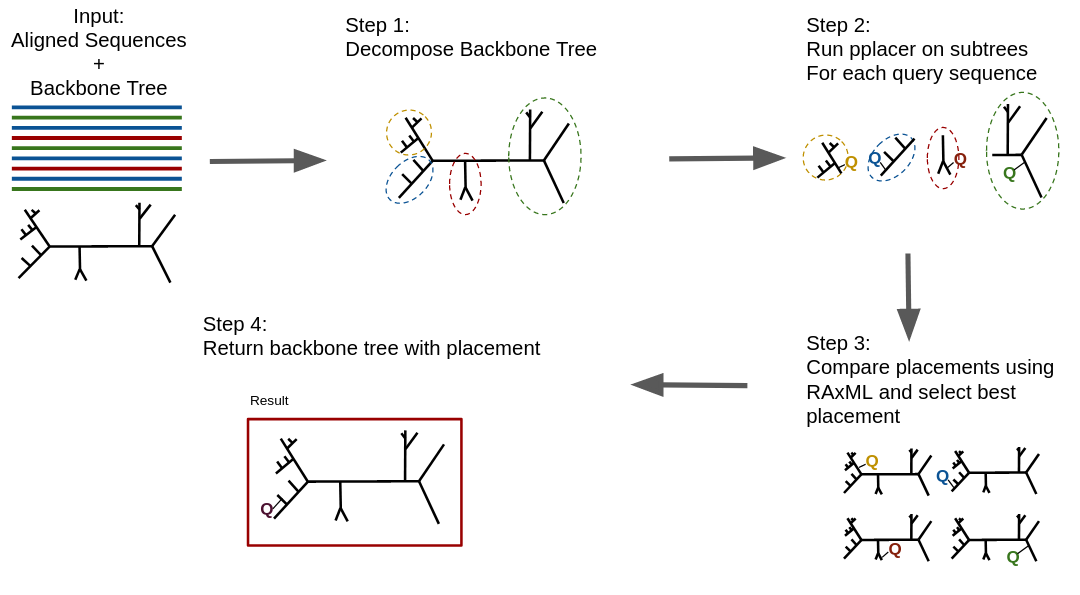
\includegraphics[width=\textwidth]{Figs/pplacerDCpipeline.png}
\label{fig:pplacerDC-pipeline}
\caption{Pipeline for pplacerDC approach
}
\end{figure}

\begin{algorithm}[H]
\SetKwFor{ParallelFor}{parallel for}{do}{endfor}
\SetAlgoLined
\KwResult{$T'$, tree T with query sequence $q$ added}
\KwIn{Tree $T$ on $N$ sequences, the MSA of $N+1$ sequences, and query sequence $q$}
 // $\operatorname{centroidDecomposition}$ decomposes a tree into roughly equal size, disjoint parts until the trees are no larger than the prescribed size.\;
 // $\operatorname{modifyTree}$ adds sequence to a tree based on the sequence's location in the a subtree with the sequence added\;
 $\{T_1,\dots,T_n\} \leftarrow \operatorname{centroidDecomposition}(T,1000)$\;
 $\{S_1, \dots, S_n\} \leftarrow 0$ // Score for each tree\;
 \ParallelFor{$i=1,\dots,n$}{
  // Place query sequence $q$ into the subtree\;
  $T'_i \leftarrow \operatorname{pplacer}(T_i, q)$\;
  // Add the location of the query sequence $q$ to a copy of $T$\;
  $T_{q_{i}} \leftarrow \operatorname{modifyTree}(T, T'_i, q)$\;
  // $\operatorname{RAxMLScorer}$ runs RAxML in fixed tree mode.\;
  // The output score is the maximum likelihood found on the tree.\;
  $S_i \leftarrow \operatorname{RAxMLScorer}( T_{q_{i}})$\;
 }
 // Do a maxLoc reduction for the tree\;
 $bestTreeIndex \leftarrow \operatorname{argmax}_{i} (S_1,\dots,S_n)$\;
 return $T'_{q_{bestTreeIndex}}$\;
 \caption{divide-and-conquer pplacer}
 \label{alg:approach1}
\end{algorithm}

\subsection{pplacerAPPLES}

The second method combines APPLES and pplacer, aiming to achieve the accuracy of pplacer with the scalability of APPLES. First, it runs APPLES with the query sequence and full backbone tree. Then, it selects one or more subtrees with a limited number of leaves. The number of subtrees to use and the maximum size of the subtrees is selected through the command line. As for pplacerDC, the maximum size of the subtree should be selected to be small enough to be handled by pplacer. Then, it will use pplacer for query placement in each of the subtrees. Finally, it compares the placements in the context of the full tree using raxml-ng, as in the first approach. It not only compares each of the pplacer placements, but also the placement from APPLES.

\begin{figure}[h]
\centering
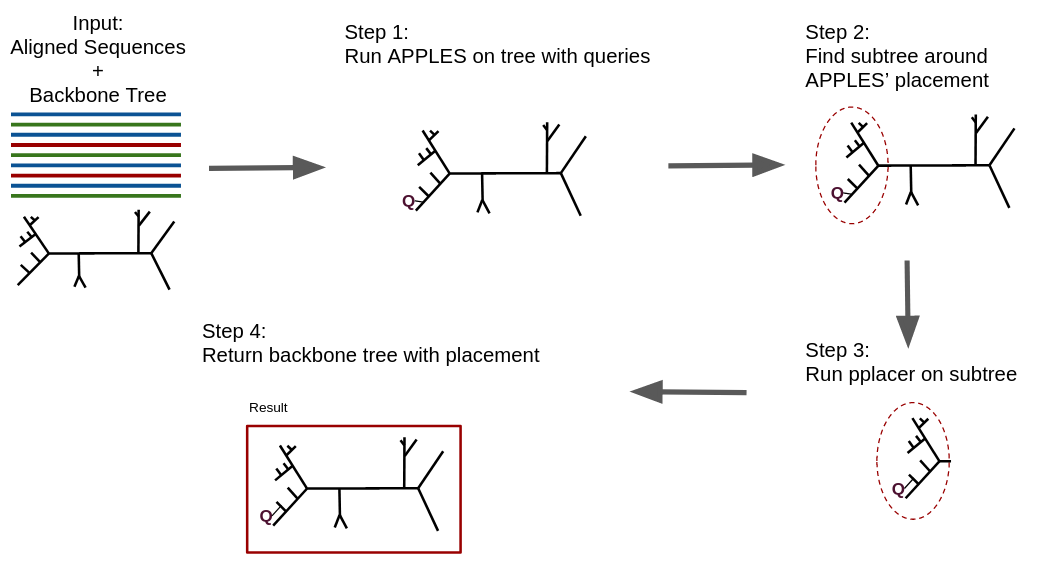
\includegraphics[width=\textwidth]{Figs/pplacerAPPLESpipeline.png}
\label{fig:pplacerAPPLES-pipeline}
\caption{Pipeline for pplacerAPPLES approach
}
\end{figure}

\begin{algorithm}[H]
\SetKwFor{ParallelFor}{parallel for}{do}{endfor}
\SetAlgoLined
\KwResult{$T'$, tree T with query sequence $q$ added}
\KwIn{Tree $T$ on $N$ sequences, the MSA of $N+1$ sequences, query sequence $q$,
and the number of clades considered, $N_{clades}$.
}
 // $\operatorname{modifyTree}$ adds sequence to a tree based on the sequence's location in the a subtree with the sequence added\;
 // $\operatorname{getRegion}$ finds a subtree containing the sequence with a maximum number of sequences\;
  // Run APPLES\;
  $T'_{APPLES} \leftarrow \operatorname{APPLES}(T, q)$\;
  // It could be the case that APPLES produces the best score\;
  $S_{apples} \leftarrow \operatorname{RAxMLScorer}( T'_{apples})$\;
  $\{S_1, \dots, S_{N_{clades}}\} \leftarrow 0$ // Score for each clade\;
  \ParallelFor{$i=1,\dots, N_{clades}$}{
    // Identify (random) region of T where q was placed with fewer than 1000 sequences\;
    $T_{i} \leftarrow \operatorname{getRegion}(T'_{APPLES}, q, 1000)$\;
    // Run pplacer on the area of T around the placement of q\;
    $T'_{pplacer} \leftarrow \operatorname{pplacer}(T_{i})$\;
  // Add the location of the query sequence $q$ to a copy of $T$\;
  $T_{q_{i}} \leftarrow \operatorname{modifyTree}(T, T_{i}, q)$\;
  // $\operatorname{RAxMLScorer}$ runs RAxML in fixed tree mode.\;
  // The output score is the maximum likelihood found on the tree.\;
  $S_i \leftarrow \operatorname{RAxMLScorer}( T_{q_{i}})$\;
  }
 // Do a maxLoc reduction for the tree\;
 $bestTreeIndex \leftarrow \operatorname{argmax}_{i} (S_{apples},S_1,\dots,S_n)$\;
 return $T'_{q_{bestTreeIndex}}$\;
\caption{APPLES with pplacer}
 \label{alg:approach2}
\end{algorithm}

\section{Results}

\begin{figure}[h]
\centering
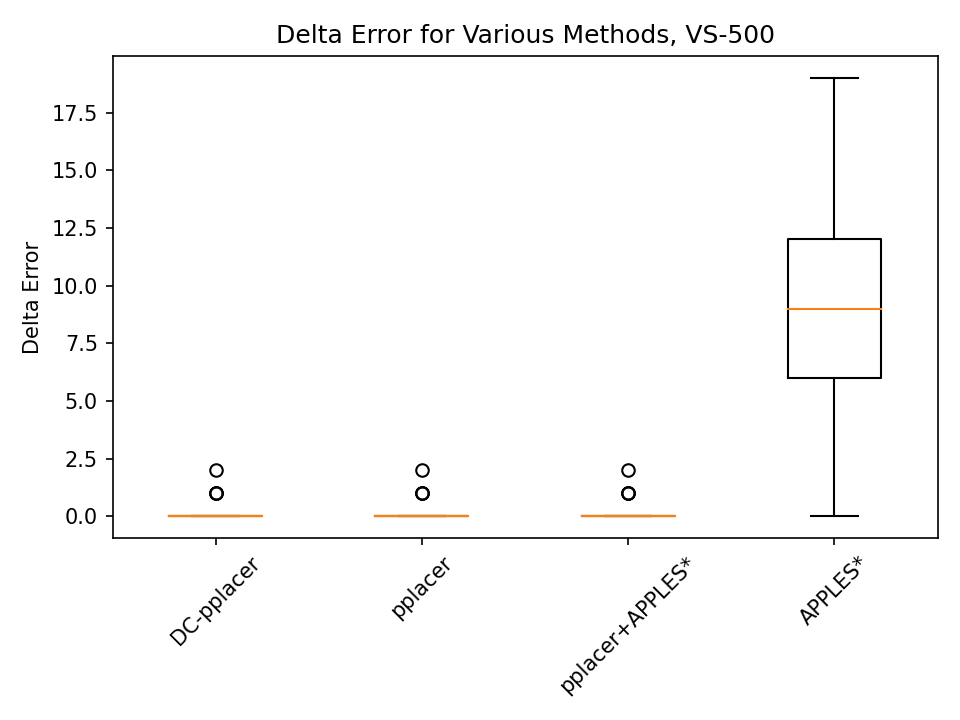
\includegraphics[width=\textwidth]{Figs/VS-delta-error-500.png}
\label{fig:error500}
\caption{Delta Error for RNASim-VS with 500 sequences}
\end{figure}

\begin{figure}[h]
\centering
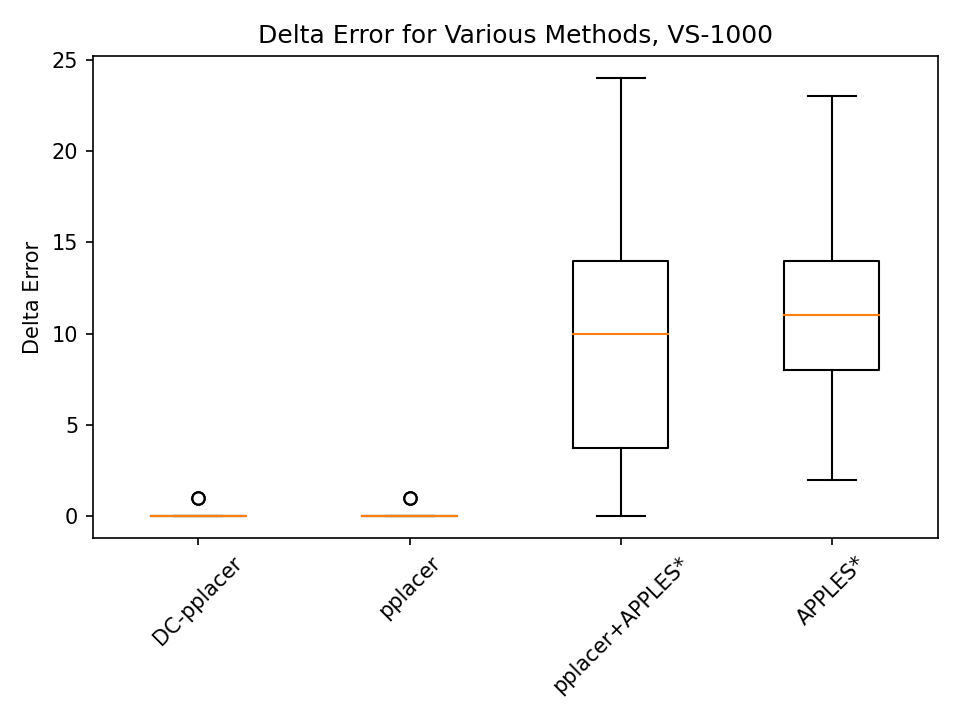
\includegraphics[width=\textwidth]{Figs/VS-delta-error-1000.png}
\label{fig:error1000}
\caption{Delta Error for RNASim-VS with 1000 sequences}
\end{figure}

\begin{figure}[h]
\centering
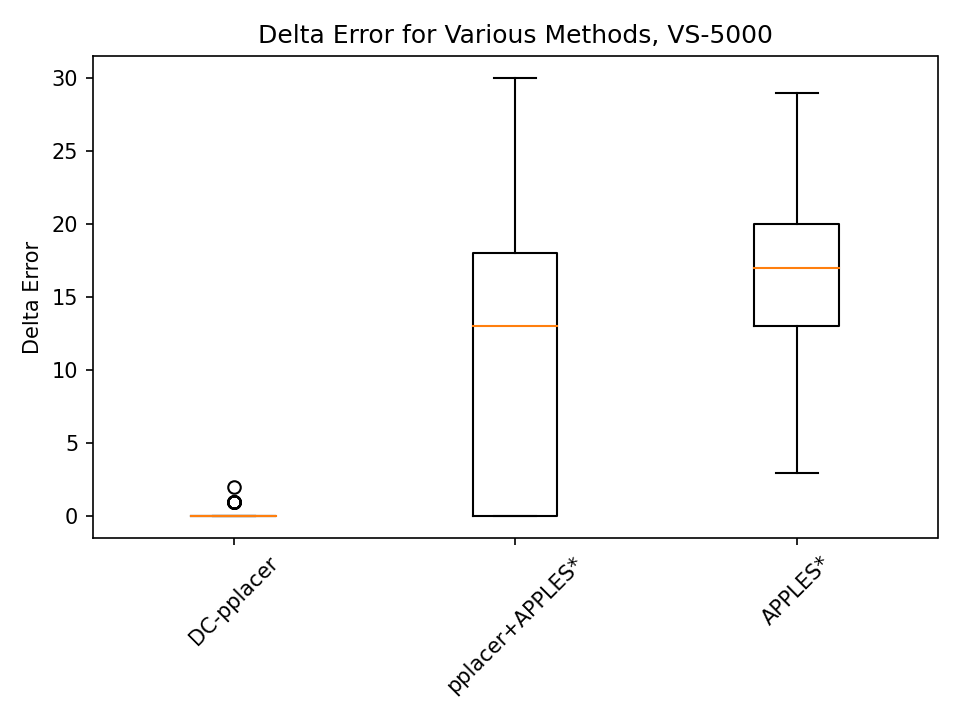
\includegraphics[width=\textwidth]{Figs/VS-delta-error-5000.png}
\label{fig:error5000}
\caption{Delta Error for RNASim-VS with 5000 sequences}
\end{figure}

\begin{figure}[h]
\centering
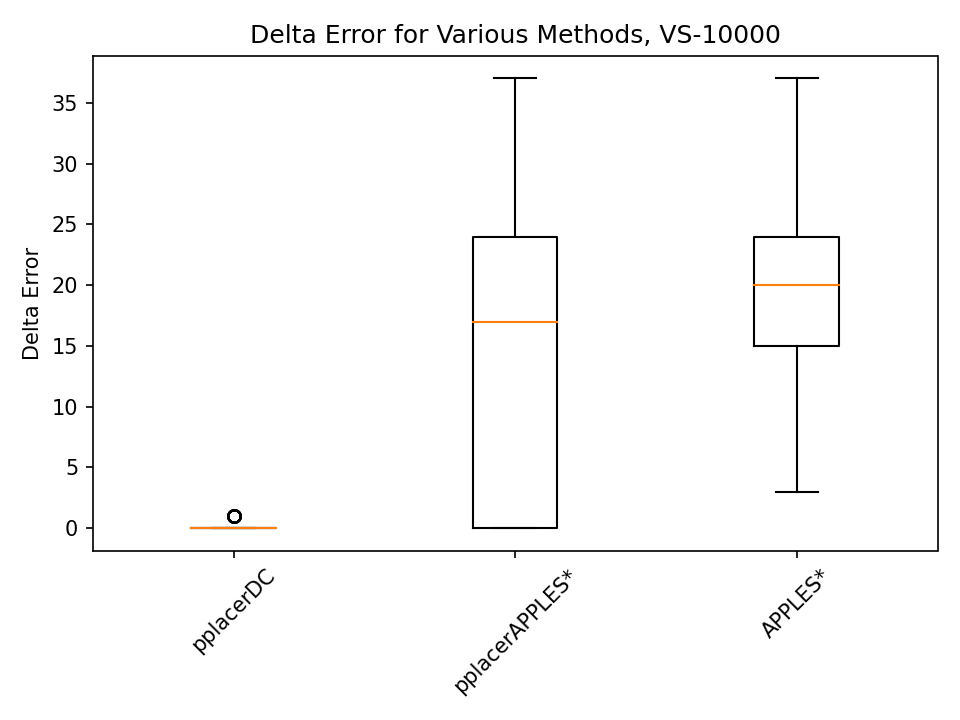
\includegraphics[width=\textwidth]{Figs/VS-delta-error-10000.png}
\label{fig:error10000}
\caption{Delta Error for RNASim-VS with 10,000 sequences}
\end{figure}

\begin{figure}[h]
\centering
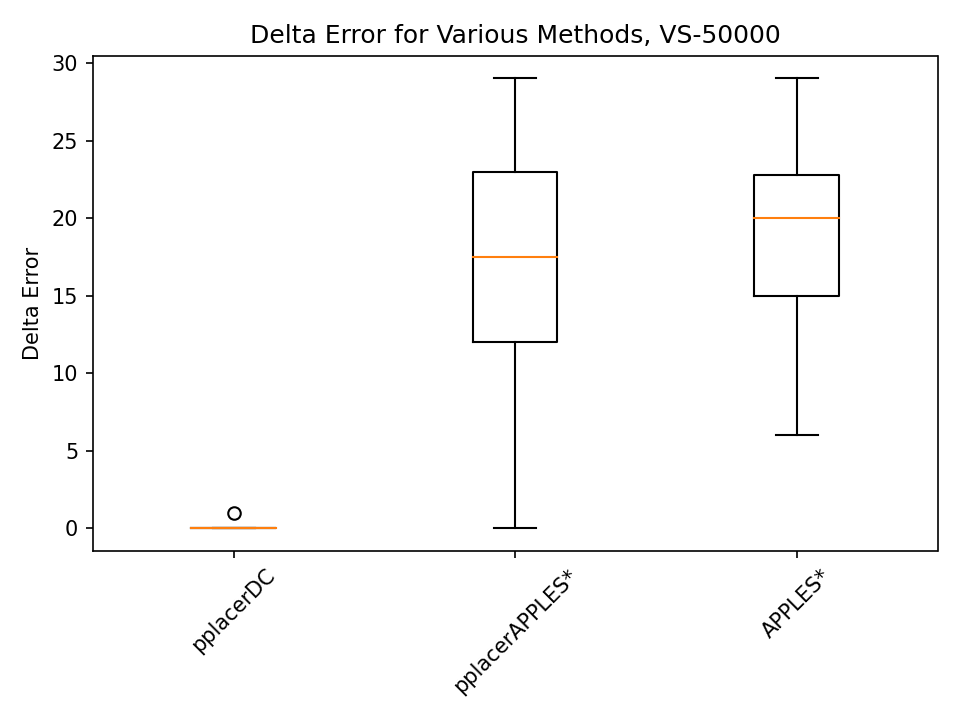
\includegraphics[width=\textwidth]{Figs/VS-delta-error-50000.png}
\label{fig:error50000}
\caption{Delta Error for RNASim-VS with 50,000 sequences}
\end{figure}

%\begin{figure}[h]
%\centering
%\includegraphics[width=\textwidth]{Figs/VS-delta-error-100000.png}
%\label{fig:error100000}
%\caption{Delta Error for RNASim-VS with 100,000 sequences}
%\end{figure}

%\begin{figure}[h]
%\centering
%\includegraphics[width=\textwidth]{Figs/VS-delta-error-200000.png}
%\label{fig:error200000}
%\caption{Delta Error for RNASim-VS with 200,000 sequences}
%\end{figure}

% TODO: update all figures to use Blue Waters results

% TODO: include discussion of all results

Through the experiments, we found that pplacerDC was significantly more accurate than APPLES for the datasets we tested on.

% TODO: expand this section a lot

\section{Discussion}

% TODO: write this section

\section{Conclusions}

% TODO: write this section

\bibliographystyle{ieee}
\bibliography{cs581-project}

\end{document}